%%%%%%%%%%%%%%%%%%%%%%%%%%%%%%%%%%%%%%%%%%%%%%%%%%%%%%%%%%%%%%%%%%%%%%%%%%%%%%%%
%2345678901234567890123456789012345678901234567890123456789012345678901234567890
%        1         2         3         4         5         6         7         8

% \documentclass[letterpaper, 10 pt, conference]{ieeeconf}  % Comment this line out if you need a4paper

\documentclass[a4paper, 10pt, conference]{ieeeconf}      % Use this line for a4 paper

\IEEEoverridecommandlockouts                              % This command is only needed if 
                                                          % you want to use the \thanks command

\overrideIEEEmargins                                      % Needed to meet printer requirements.

% See the \addtolength command later in the file to balance the column lengths
% on the last page of the document

% The following packages can be found on http:\\www.ctan.org
\usepackage{graphicx} % for pdf, bitmapped graphics files
% \DeclareGraphicsExtensions{.pdf,.jpeg,.png}
%\usepackage{epsfig} % for postscript graphics files
%\usepackage{mathptmx} % assumes new font selection scheme installed
%\usepackage{times} % assumes new font selection scheme installed
\usepackage{amsmath} % assumes amsmath package installed
\usepackage{amssymb}  % assumes amsmath package installed
% \usepackage{multicol}
% \usepackage{multirow}
\usepackage[caption=false,font=footnotesize]{subfig}
\DeclareMathOperator*{\argmax}{arg\,max}
\DeclareMathOperator*{\sgn}{sgn}


\title{\LARGE \bf
Traffic Signal Control for Isolated Intersection Based on Coordination Game and Pareto Efficiency*
}


\author{Yang Zhao$^{1}$ and Jianming Hu$^{2}$, \IEEEmembership{Member, IEEE}% <-this % stops a space
\thanks{*This work was supported by any organization}% <-this % stops a space
\thanks{$^{1}$Yang Zhao is with Department of Automation,
        Tsinghua University, 100084 Beijing, China
        {\tt\small zhaoy-18@mails.tsinghua.edu.cn}}%
\thanks{$^{2}$Jianming Hu is with Department of Automation,
        Tsinghua University, 100084 Beijing, China
        {\tt\small hujm@mail.tsinghua.edu.cn}}%
}


\begin{document}



\maketitle
\thispagestyle{empty}
\pagestyle{empty}


%%%%%%%%%%%%%%%%%%%%%%%%%%%%%%%%%%%%%%%%%%%%%%%%%%%%%%%%%%%%%%%%%%%%%%%%%%%%%%%%
\begin{abstract}
Nowadays, with the rapid increasement of the vehicles number, traffic congestion becomes a severe problem in almost every city. 
The applications of Intelligent Transportation Systems makes it possible for a signal control system to collect real-time data 
of an intersection, helping to improve the traffic signal control strategy and traffic efficiency. This paper proposes an algorithm 
based on coordination game and Pareto efficiency, by using vehicles position, speed and acceleration information, 
to control traffic signal for an isolated intersection in real time. The proposed algorithm is simulated on the SUMO 
microscopic traffic simulation platform and compared to a Webster's fixed-time plan and an actuated control algorithm to 
evaluate the performance in different traffic flow. The simulation results demonstrate that the algorithm based on coordination
game and Pareto efficiency is more efficient than the Webster's fixed-time plan and actuated control algorithm in average queue 
length, average total delay and average travel time. 
\end{abstract}


%%%%%%%%%%%%%%%%%%%%%%%%%%%%%%%%%%%%%%%%%%%%%%%%%%%%%%%%%%%%%%%%%%%%%%%%%%%%%%%%
% ===========================================================================
%  section 1 introduction
% ===========================================================================
\section{INTRODUCTION}
With the development of the economy, the number of vehicles increase rapidly, causing a severe traffic congestion problem. 
The intersection plays a critical role in urban traffic system, so an efficient traffic control strategy can really ease the traffic
pressure. However, the existing urban traffic signal control (TSC) systems cannot fully achieve the requirements of the optimal 
traffic control. Hence, it is necessary to design a time-variant TSC system to adjust the real-time traffic demand. 
The theoretical research of the TSC algorithm could date back to 1950s. From then on, TSC algorithms proposed by many researchers could 
be categorized as one of the following: fixed-time plan (FP), actuated method (ACT) and adaptive algorithm \cite{zhao2012computational}.

The FP, using the predetermined time cycle and green duration for each phase, does not consider the real-time traffic data. Therefore, it 
is suitable for the relatively stable and regular traffic flows. The most famous FP method is proposed by Webster in 
1958. This formula based on the flow rate of each lane in an intersection
is useful to find an optimal cycle and appropriate duration for green time in each phase \cite{webster1958traffic}.
However, Beacuse the traffic system is a dynamic system, the FP plan cannot fit all real-time conditions. 

The ACT, also called real-time traffic-responsive control, came into practice with the help of the development of the sensor technologies. 
This method need install the vehicle detectors before the intersection stop lines. By collecting the data from the detectors, the 
signal control system will make different traffic control action under a certain control strategy based the collected real-time information.
The ACT method, choosing to change to another phase or extend the current phase duration based on
real-time traffic demand and predefined logic rules, is widely used in current traffic system. 
Though the ACT method was proved to perform better than FP method in most situations, 
it does not work when the traffic saturation is high. The extension of the current phase only depends on vehicles of the current phase, 
without considering the queue length other phases. Therefore, it cannot achieve the optimal strategy of the intersection. 

Parameters like time, day, season, weather, and many unpredictable situations such as accidents are highly influential on traffic system. 
Hence, the adaptive TSC system was creadted to take into account more information to achieve more efficient signal controller.  
Sydney coordinated adaptive traffic system (SCATS) and Split cycle offset optimization technique (SCOOT) both belongs to this category. 
SCATS detects the traffic flows and headways at the stop bars. Based on information gathered in one-minute intervals, 
green times are reallocated to the phases of greatest need. The system benefits to Sydney over fixed time control 
in terms of reduced delay, reduced accidents, fuel saved and air pollution reduction are quantified \cite{sims1981scat}.
And the SCOOT system adjusts the signal timings in frequent, small increments to match the latest traffic situation and 
is designed for general application within computerised urban traffic control systems \cite{hunt1981scoot}.

Although the adaptive method can fit different traffic situations better, it need more real-time information in the whole network. The 
limitation of traditional traffic sensors is that they are the pointed detectors that only provide instantaneous vehicle information
only when the vehicle passes the detector and cannot continuously provide the position, speed and acceleration data of the 
vehicles \cite{feng2015real}. Therefore, the Intelligent Transportation System (ITS) introduces wireless communications among smart vehicles 
and roadside infrastructure to collect continuous real-time data. Under this environment, the traffic control system can use high speed 
information transactions between vehicles, vehicles and infrastructure, rather than the sensor at fixed location, 
to get access to detailed vehicle information, such as position, speed and acceleration. 

Game theory is the study of mathematical models of strategic interactions between rational decision makers \cite{hammerstein1994game}. It has
applications in all fields of social science, military, as well as in logic and computer science. In the field of the transportation, game 
theory has been applid to traffic flow optimization \cite{bui2018cooperative}, cooperative adaptive cruise control 
systems \cite{zohdy2012game}, intersection traffic control \cite{elhenawy2015intersection} and route guidance \cite{jun2003study}.
Besides, Game theory is considered a suitable method to solve the intersection traffic signal control problem \cite{abdelghaffar2016isolated}. 

In this paper, we propose an isolated intersection traffic signal control algorithm based on coordination game. We will view each phase of the 
isolated interaction as the game player and use the estimated queue length as reward function. This algorithm is a cycle-free control strategy. 
To consider all phase reward at the same time, we will view all the rewards as a vector and choose the optimal action using Pareto efficiency. 
The game theory based algorithm is then simulated on the SUMO \cite{SUMO2012} microscopic traffic simulation platform and compared to the 
Webster's FP and ACT. To evaluate the performance of the game theory based algorithm, average queue length, average total delay and average
travel time will be caculated. 

The rest of this paper is organized as follows. In section \uppercase\expandafter{\romannumeral2}, we will review briefly for some game theory 
based signal controllers. In section \uppercase\expandafter{\romannumeral3}, we will introduce the signal control model based on coordination
game and describe how to control a signalized intersection under the game theory based algorithm. In section \uppercase\expandafter{\romannumeral4},
the simulation will be shown and we will discuss and summarize the results of the simulation. In section \uppercase\expandafter{\romannumeral5}, 
we will conclude the whole paper. 
% ===========================================================================
%  section 2 related work
% ===========================================================================
\section{RELATED WORK}

In order to minimize the queue length and to maximize the intersection efficiency, many approaches are proposed to solve the TSC problem. 
Game theory, the basic theory of coordinating the actions of intersection controllers, has been introduced into traffic coordinated
control problem in recent years. In 1995, Bazan et al. \cite{bazan1995game} viewed the intersection as twp-player games in which 
agents have different and incomplete knowledge and update their beliefs with time. 
In 2003, the theory of differential game is used to model the TSC system \cite{zhen2003differential}. 
In this paper, dynamic trafic assignment and trafic signal control are formulated as a leader-follower differential game, in which a leader and
multi-follower participate, under the open-loop information structure. After that, Villalobos et al. \cite{villalobos2008urban} proposed a 
noncooperative game model for signal control problem and solved the model using $\epsilon$-Nash equilibrium and Extraproximal method. 

Besides the noncooperative game model, which may suffer from the local optimal solution, 
Tan et al. \cite{linglong2010study} were the first to use Nash bargaining to optimize a two-phase traffic 
signal, which was modeled by a twp-player coordination game model. In 2016, Hossam M. Abdelghaffar et al. \cite{abdelghaffar2016isolated} develop 
the Nash bargaining algorithm, which uses a cycle-free control strategy to optimize four-phase isolated signalized intersection traffic signal timings. 

Moreover, Xia Xinhai et al. \cite{xinhai2009traffic} combined the game theory and reinforcement learning to propose a traffic signal control agent 
interaction model. Dong et al. \cite{dong2011multi} \cite{dai2013multi} applied the game theoretic framework for the multi-intersection. 

However, most of these work only consider two-phase information at one time, which may lead to the local optimal solution. Another limitation of 
current game theory based algorithm is that they used either noncooperative game model or cooperative model. Our work will model the four-phase
isolated intersection with noncooperative game framework and solve it by using Pareto efficiency, which is a concept from cooperative game model, to 
guanrantee the solution is at least Pareto Optimality.

% ===========================================================================
%  section 3 signal control model based on coordination game
% ===========================================================================
\section{SIGNAL CONTROL MODEL BASED ON COORDINATION GAME}

In this section, we will describe the coordination game model and Pareto efficiency solution for two players, which is shown in section 
\uppercase\expandafter{\romannumeral3}-A, and the four-phase traffic signal model based on coordination game, as is shown in section 
\uppercase\expandafter{\romannumeral3}-B. 

\subsection{Two-Player Coordination Game and Pareto Efficiency Solution}
In game theory, coordination games are a class of games with multiple pure strategy Nash equilibrium in which players choose the same or corresponding 
strategies \cite{osborne1994course}. When a game is a coordination game, the following inequalities hold in the payoff matrix shown in Table 
\ref{Tab:PayMatrix}. For player $P_1$, $R_1>R_3$ and $R_4>R_2$, and for player $P_2$, $r_1>r_2$ and $r_4>r_3$. This means strategy profiles $(A_1, a_1)$
and $(A_2,a_2)$ are pure Nash equilibrium and this can be extend to more than two players. 

\begin{table}[h]
        \caption{TWO PLAYERS PAYOFF MATRIX}
        \label{Tab:PayMatrix}
        \begin{center}
                \begin{tabular}{|c|c|c|}
                        \hline
                        &$P_2(a_1)$&$P_2(a_2)$\\
                        \hline
                        $P_1(A_1)$&$(R_1,r_1)$&$(R_2,r_2)$\\
                        \hline
                        $P_1(A_2)$&$(R_3,r_3)$&$(R_4,r_4)$\\
                        \hline
                \end{tabular}
        \end{center}
\end{table}

If $R_1>R_4$ and $r_1>r_4$, we say $(R_1,r_1)$ Pareto dominates the $(R_4,r_4)$ (of coures it also Pareto dominates the $(R_2,r_2)$ and the $(R_3,r_3)$). Thus, 
the best action pairs is $(A_1,a_1)$ though the game still have two pure Nash equilibrium. In this situation, we say the $(A_1,a_1)$ is Pareto efficiency
solution. Similarly, if $R_4>R_1$ and $r_4>r_1$, the $(A_2,a_2)$ is the Pareto efficiency solution. 

However, in most situations, we will have $R_1>R_4$, $r_1<r_4$ or $R_1<R_4$, $r_1>r_4$, which means it is hard to say which action pair is more
efficient. To solve this problem, mixed strategy Nash equilibrium was proposed. For the coordination game above, a mixed Nash equilibrium is given by 
a probability $p$ to play $A_1$ and $1-p$ to play $A_2$ for player $P_1$, and another probability $q$ to play $a_1$ and $1-q$ to play $a_2$ for player 
$P_2$, where $p$ and $q$ can be caculated as (\ref{eq:p}) and (\ref{eq:q}).
\begin{align}
        \label{eq:p}
        p&=\frac{r_4-r_3}{r_1-r_2-r_3+r_4}\\
        \label{eq:q}
        q&=\frac{R_4-R_2}{R_1-R_2-R_3+R_4}
\end{align}

Unfortunately, this solution is not good enough. On one hand, the mixed Nash equilibrium solution is Pareto dominated by the two pure Nash equilibrium since 
the players will fail to coordinate. On the other hand, the solution is useful when the coordination game is also a repeat game, but in our model, it is not. 

In our situation, the controller can be viewed as a traffic management who aims to reduce the vehicle queue length. That means we can choose the 
Pareto solution in the payoff matrix to get the largest payoff in the whole system. To get the Pareto solution, for every action pair $(A,a)$, we 
define the objective function as the weighted sum of payoff of all players under this action pair, i.e:
\begin{equation}
        W(A,a)=w_1u_1(A,a)+w_2u_2(A,a)
\end{equation}
where $u_i(a_1,a_2)$ is the payoff of player $i$ when the player 1 chooses the action $a_1$ and player 2 chooses the action $a_2$ 
and $w_1,w_2\ge 0$ are predefined, determining which player is more important. The Pareto solution can be obtained by solve 
the following optimization problem, i.e:
\begin{equation}
        \label{eq:op}
        (A^*,a^*)=\argmax\limits_{(A,a)} W(A,a)
\end{equation}

Besides, we also do not want to let one player's benefit is much larger than the others'. We introduce the reject region bounded by two line 
passing through the $(0,0)$ and we would ignore the Pareto solution in the rejcet region. 
The geometry interpretation of (\ref{eq:op}) is shown in Fig \ref{fig:Pareto}.
\begin{figure}[thbp]
        \centering
        \subfloat[][]{\label{Fig:11}
        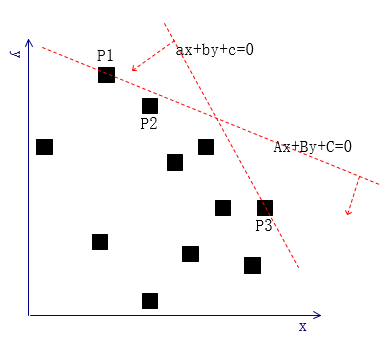
\includegraphics[width=1.6in]{figures/Pareto.PNG}}\hfill
        \subfloat[][]{\label{Fig:12}
        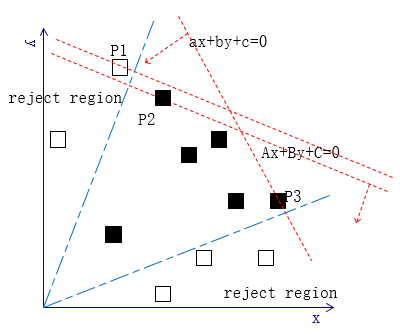
\includegraphics[width=1.6in]{figures/Pareto_rej.PNG}}\par
        \caption{The geometry interpretation for the Pareto solution. 
        \ref{Fig:11} shows that P1 and P3 is the different solution under different non-nagetive weights. But in \ref{Fig:12}, 
        the P1 is in the rejcet region bounded by the two blue line, so the real solution is the P2 if we choose $(A,B)$ as the weights.}
        \label{fig:Pareto}
\end{figure}

In our case, the weights represent our 
preference to choose keep action or switch action, and the reject region will balance the queue length for each phase. 

\subsection{Four-Phase Traffic Signal Model Based on Coordination Game}
For four-phase isolated intersection, we use the standard NEMA phasing as shown in Fig. \ref{fig:NEMA}. And the yellow time for each phase 
is predefined as 3 seconds.
\begin{figure}[thpb]
        \centering
        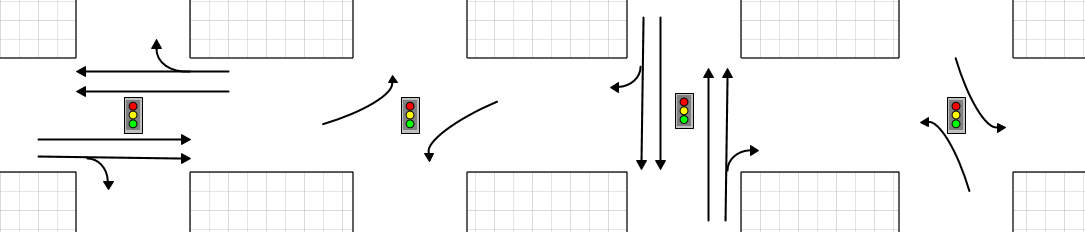
\includegraphics[width=3.3in]{figures/NEMA.PNG}
        %\includegraphics[scale=1.0]{figurefile}
        \caption{Standard NEMA phasing}
        \label{fig:NEMA}
\end{figure}
According to game theory, we will define the game players, strategies and reward functions as follow:
\begin{itemize}
        \item \textbf{Players:} All four phases, denoted by $P_1,P_2,P_3,P_4$, where $P_1$ represents the current green phase. 
        In the period of signal cycle, every second in green 
        time will have a non-cooperative game process and controller will choose the corresponding action.
        \item \textbf{Strategies:} Keep current phase, $A_1$, or change to next phase, $A_2$. Firstly, we must note that the phase cannot be 
        kept all the time. To avoid this situation, 
        we predefine the minimum green time for each phase as 5 seconds and the maximum green time for each phase as 30 seconds. 
        Every phase in a signal cycle
        will at least obatins minimum green time and at most obatins maximum green time. Secondly, in the meanwhile, the system can only have one green phase, which
        means if one player choose to keep, others must also choose to keep and vice versa. Thus, the strategy profiles $(keep,keep,keep,keep)$ and 
        $(change,change,change,change)$ are two pure Nash equilibrium. And that is why this model is based on coordination game.
        \item \textbf{Payoff functions:} Estimated queue length of each phase in a few time interval after applying a specific action, denoted by $R_P(t,\Delta t)$. 
        This measurement can be estimated if we know position, speed and acceleration of all vehicles in SUMO. 
\end{itemize}

The reward function for each player (phase) is caculated as the following equation:
\begin{equation}
        R_P(t,\Delta t)=\max\limits_{l\in P}\{q_l(t)+A_l(t,\Delta t)-D_l(t,\Delta t)\}
\end{equation}
where $l$ is the corresponding lane for each player, $q_l(t)$ is the current queue length (number of vehicle) associated with corresponding lane 
$l$ at time $t$, $A_l(t,\Delta t)$ is the estimated number of arrival vehicle in lane $l$ between the time interval $[t,t+\Delta t]$, $D_l(t,\Delta t)$
is the estimated number of departure vehicles in lane $l$ between the time interval $[t,t+\Delta t]$, $D_l(t,\Delta t)$. 

In SUMO, if the vehicle $i$ speed $v_i^t$ is less than a predefined threshold speed $v_{th}$ at time $t$ and the distance $d_i^t$ to the intersection
is less than a predefined threshold distance $d_{th}$, we will view this vehicle is in queue. Thus, 
\begin{equation}
        q_l(t)=\sum_{i\in l}n_i^t
\end{equation}
\begin{equation}
        n_i^t=\begin{cases}
                1&\quad\text{if}\,v_i^t<v_{th}\,\text{and}\,d_i^t<d_{th}\\
                0&\quad\text{else}
        \end{cases}
\end{equation}

For $A_l(t,\Delta t)$, we will use the kinematics formulas to estimate as (\ref{eq:arrival}), where $\sgn(x)$ is the symbolic function.
\begin{equation}
        \label{eq:arrival}
        A_l(t,\Delta t)=\sum_{i\in l}\sgn(\min\{0,\Delta t-\frac{v_i^t}{a_i^t}\})
\end{equation}

For $D_l(t,\Delta t)$, the caculation could be split into three conditions. For the phase which is in green phase and hope to keep the current
phase (condition $c_1$), we could simply use the saturation flow rate to estimate; for the phase which is in red phase and hope to switch to the 
green phase (condition $c_2$), we could not use the saturation flow rate (the green phase will just begin), so we will use kinematics formulas
to estimate; for the else condition, the number of departure vehicle is zero. Hence, the formula of the $D_l(t,\Delta t)$ is shown as 
the (\ref{eq:departure}):
\begin{equation}
        \label{eq:departure}
        D_l(t,\Delta t)=\begin{cases}
                Q_{sl}\Delta t&\text{for cond}\, c_1\\
                \sum_{i\in l}\sgn(\max\{0,\Delta L\})&\text{for cond}\, c_2\\
                0&\text{else}
        \end{cases}
\end{equation}
where $Q_{st}$ is the saturation flow rate for lane $l$, $\Delta L$ could be estimated as follow:
\begin{equation}
        \Delta L=v_i^t(\Delta t-t^y)+\frac{1}{2}a_i^t(\Delta t-t^y)^2-d_i^t
\end{equation}
where $t^y$ is the yellow light duration. 

To solve the four players coordination game, we can view the $P_2,P_3,P_4$ as a cooperative player $P_c$ who wants to choose switch action, and 
the payoff function could be caculated by 
\begin{equation}
        R_{p_c}(t,\Delta t)=aR_{p_2}(t,\Delta t)+bR_{p_3}(t,\Delta t)+cR_{p_4}(t,\Delta t)
\end{equation}
where $a,b,c\ge 0$ satisfy
\begin{equation}
        a+b+c=1
\end{equation}
Hence, this problem is converted to the two-player coordination game and can be solved by the Pareto efficiency based method introduced 
in section \uppercase\expandafter{\romannumeral3}-A.

\section{SIMULATION AND RESULTS}

In this section, we will describe the simulation and the results. Section \uppercase\expandafter{\romannumeral4}-A introduces the 
test intersection. Section \uppercase\expandafter{\romannumeral4}-B describes the measures of effectiveness and simulation parameters and 
section \uppercase\expandafter{\romannumeral4}-C is the results of the experiments and our discussion.

\subsection{Test Intersection}
\begin{figure}[thpb]
        \centering
        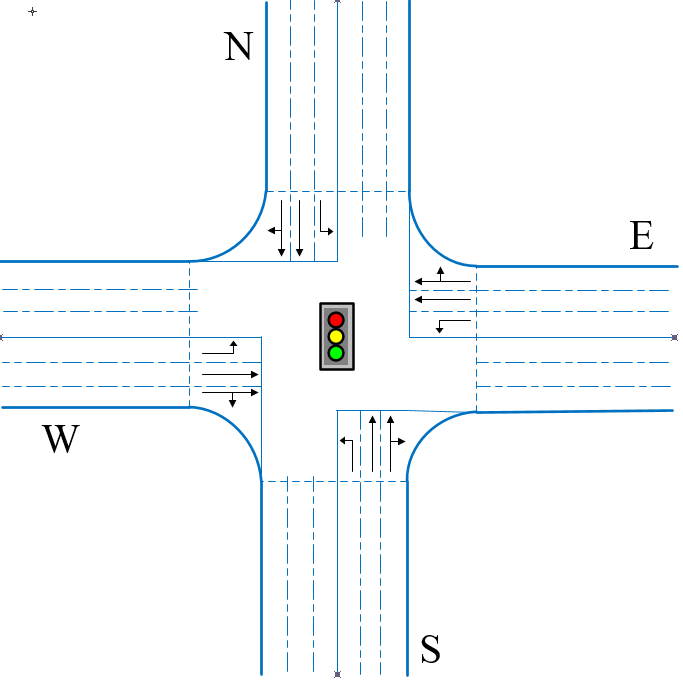
\includegraphics[width=2.3in]{figures/Intersection.PNG}
        %\includegraphics[scale=1.0]{figurefile}
        \caption{Test Intersection.}
        \label{fig:Intersection}
\end{figure}

The simulation will be tested on an intersection with four roads comprised of three lanes each, as shown in Fig \ref{fig:Intersection}.


The traffic demand origin-destination (O-D) matrix is provided in Table \ref{Tab:ODMatrix}, which are set in the SUMO simulation platform.
\begin{table}[h]
        \caption{O-D traffic demand matrix}
        \label{Tab:ODMatrix}
        \begin{center}
                \begin{tabular}{|c|c|c|c|c|c|}
                        \hline
                        Zone&W&E&N&S&Total\\
                        \hline
                        W&-&900&225&225&1350\\
                        \hline
                        E&900&-&225&225&1350\\
                        \hline
                        N&113&113&-&450&676\\
                        \hline
                        S&113&113&450&-&676\\
                        \hline
                        Total&1123&1123&900&900&4046\\
                        \hline
                \end{tabular}
        \end{center}
\end{table}



\subsection{Measures of Effectiveness and Simulation Parameters}
The following measures of effectiveness (MOE) are used to evaluate the performance of our algorithm, Webster's FP and ACT method. 
\begin{itemize}
        \item \textbf{Average Queue Length (veh):} the sum of the vehicles in queue for each lane each second divied by the simulation duration 
        and number of the lane. 
        \item \textbf{Average Travel Time (s/veh):} the sum of all vehicles' travel time divied by the number of vehicles.
        \item \textbf{Average Total Delay (s/veh):} the sum of all vehicles' delay divied by the number of vehicles.
\end{itemize}

The important simulation parameters' value are set as follow:
\begin{align*}
        &\text{Threshold speed}\, s_{th}=3.6\,\text{(km/h)}\\
        &\text{Threshold distance}\, d_{th}=100\,\text{(m)}\\
        &\text{Saturation flow rate}\, Q_{sl}=1650\,\text{(veh/h/lane)}\\
        &\text{Yellow time}\, t^y=3\,\text{(s)}\\
        &\text{Max vehicle speed}\, v_{max}=50\,\text{(km/h)}\\
        &\text{Max green time}\, t^g_{max}=30\,\text{(s)}\\
        &\text{Min green time}\, t^g_{min}=5\,\text{(s)}
\end{align*} 

\subsection{Results and Discussion}

The Webster's FP and the ACT method will be used as the base line to evaluate the performance of our approach. Three scenarios are 
simulated: one for the orignal O-D matrix shown in Tabel \ref{Tab:ODMatrix}; second is for a lower demand which is the demand of $80\%$ of
the orignal O-D matrix; the last is for a higher demand which is the demand of $120\%$ of the orignal O-D matrix. 

First, we will study the effect for the different time interval $\Delta t$ under the orignal O-D matrix demand. Beacuse our yellow time for 
each phase is set as 3 seconds and the max green time $t_{max}^g$ is set as 30 seconds, the $\Delta t$ is set to vary from 5 seconds to 25 seconds.
To evaluate the performance, we use the results of the Webster's FP as the reference and the experiments' results are shown as Fig \ref{fig:RESt}.

\begin{figure*}[thbp]
        \centering
        \subfloat[][]{\label{Fig:11}
        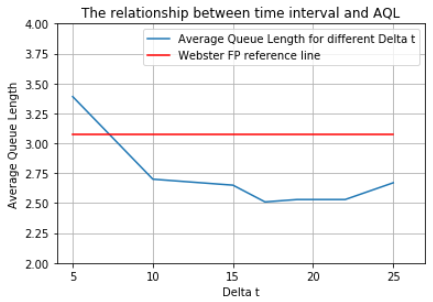
\includegraphics[width=2.0in]{figures/AQLt.PNG}}\hfill
        \subfloat[][]{\label{Fig:12}
        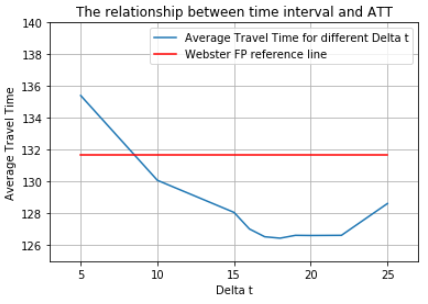
\includegraphics[width=2.0in]{figures/ATTt.PNG}}\hfill
        \subfloat[][]{\label{Fig:13}
        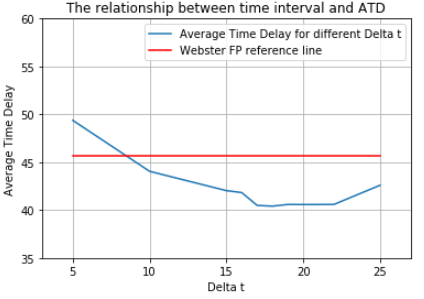
\includegraphics[width=2.0in]{figures/ATDt.PNG}}\par
        \caption{The results of simulation for different $\Delta t$ and different measurements under the orignal traffic demand. 
        The red line is a reference results obtained by the Webster's FP.
        \ref{Fig:11} shows the relationship between $\Delta t$ and the average queue length. 
        \ref{Fig:12} shows the relationship between $\Delta t$ and the average travel time.
        \ref{Fig:13} shows the relationship between $\Delta t$ and the average total delay.}
        \label{fig:RESt}
\end{figure*}
\begin{table*}[h]
        \caption{MOE for different traffic demand and different methods}
        \label{Tab:Res}
        \begin{center}
                \begin{tabular}{|c|c|c|c|c|c|c|c|c|c|}
                        \hline
                        Demand&\multicolumn{3}{c|}{Lower Demand}&\multicolumn{3}{c|}{Orignal Demand}&\multicolumn{3}{c|}{Higher Demand}\\
                        \hline
                        Method&Webster&ACT&GT&Webster&ACT&GT&Webster&ACT&GT\\
                        \hline
                        Average Queue Length (veh)&1.65&1.48&1.53&3.07&2.67&2.51&10.11&11.57&7.57\\
                        \hline
                        AQL Improvement (\%)&+7.30&-3.37&&+18.24&+5.99&&+25.12&+34.57&\\
                        \hline
                        Average Trival Time (s/veh)&119.05&116.77&117.71&131.68&127.30&126.53&211.54&233.62&193.52\\
                        \hline
                        ATT Improvemen (\%)t&+1.10&-0.08&&+3.90&+0.60&&+8.52&+17.20&\\
                        \hline
                        Average Total Delay (s/veh)&33.16&30.87&31.82&45.64&41.26&40.49&125.47&147.54&107.45\\
                        \hline
                        AQL Improvement (\%)&+4.04&-0.03&&+11.22&+1.86&&+14.36&+27.17&\\
                        \hline
                \end{tabular}
        \end{center}
\end{table*}
\begin{figure*}[thbp]
        \centering
        \subfloat[][]{\label{Fig:11}
        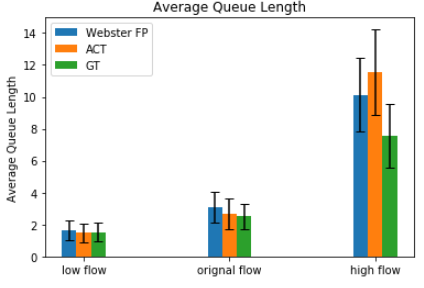
\includegraphics[width=2.0in]{figures/AQL.PNG}}\hfill
        \subfloat[][]{\label{Fig:12}
        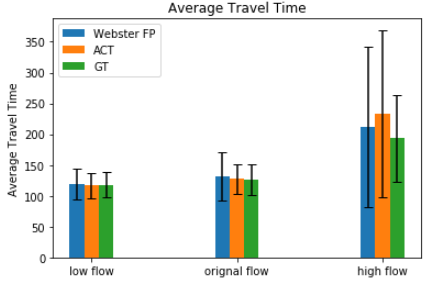
\includegraphics[width=2.0in]{figures/ATT.PNG}}\hfill
        \subfloat[][]{\label{Fig:13}
        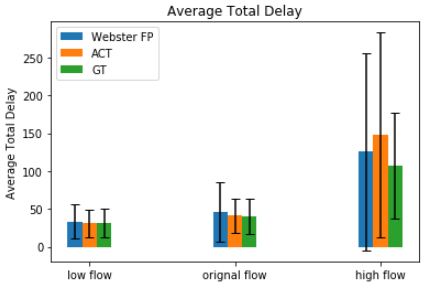
\includegraphics[width=2.0in]{figures/ATD.PNG}}\par
        \caption{The results of simulation for different methods and different measurements. 
        \ref{Fig:11} shows the average queue length and standard deviation for FP, ACT and GT under different traffic demand.
        \ref{Fig:12} shows the average travel time and standard deviation for FP, ACT and GT under different traffic demand.
        \ref{Fig:13} shows the average total delay and standard deviation for FP, ACT and GT under different traffic demand.}
        \label{fig:RES}
\end{figure*}


Fig \ref{fig:RESt} shows that our approach performs better than the Webster's FP approach for almost all the $\Delta t$ in 
average queue length, average travel time and average total delay, especially when $\Delta t$ varies from $16$ to $22$. This results 
prove that our approach is not sensitive to the parameter $\Delta t$. 

Next, we will give the explaination of the results shown in Fig \ref{fig:RESt}. When $\Delta t$ is small, which means it is close to the 
yellow time, the payoff function of next phase corresponding to the switch function increase slowly for too short effective green time. 
When $\Delta t$ is large, the estimation used kinematics formulas will have large bias beacuse all the variables we use are detected at 
one moment. 

According to the results obtained above, we set the parameter $\Delta t$ as 17 to continue our experiments. 
The simulation results for different methods and different traffic demand are shown in Tabel \ref{Tab:Res}. We also caculate the improvement
of our game theory approach compared with the Webster approach and ACT method in Tabel \ref{Tab:Res}. And we can find that the average values
for all three MOE of our approach is better except the ACT approach under lower traffic demand. However, the Fig \ref{fig:RES} shows the 
average and the standard deviation for different measurement and different traffic demand and we can find that the standard deviation of our 
approach is less than the other two methods, which indicates that our approach is more stable.

To show the reason why our approach works, Fig \ref{fig:AQLEL} shows the average queue length for every lane by using Webster's FP, ACT method and 
our approach under the orignal traffic demand. It is obvious that although our approach is not the best for almost every lane, the last results 
show that our approach is the best. On the other hand, Fig \ref{fig:AQLEL} shows that the Webster's FP works better for phase with higher traffic flow
and ACT method performs better for phase with lower traffic flow, which makes the large difference between different phase under the same method.
However, for our game theory based approach, the average queue length of almost all the lane is on the same level, no matter how the level of 
traffic flow is. Hence, we can view our approach as a balanced method to guanrantee the traffic signal system is more efficient. 

\begin{figure}[thbp]
        \centering
        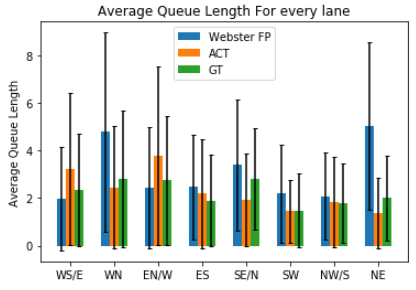
\includegraphics[width=2.8in]{figures/AQLeverylane.PNG}
        \caption{The average queue length for every lane of this test intersection for different methods under the orignal traffic demand.}
        \label{fig:AQLEL}
\end{figure}

The simulation results show that, for our coordination game method, not only the average value, but also the standard deviation are 
better than the Webster's FP and ACT method in average queue length, average travel time and average total delay. What's more, our approach
is a real-time, stable, balanced and non-sensitive to parameters traffic signal control algorithm based on the discussion above. 



\section{CONCLUSIONS}

This paper proposed a real-time coordination game based isolated intersection traffic signal control algorithm and used the SUMO simulation platform 
to evaluate this approach in a test intersection compared with the Webster's FP and ACT method in average queue length, average travel time 
and average total delay. The results show that it is possible for our approach to make the isolated intersection more efficient. Besides, 
we also discussed the effect of the parameter in our approach and gave the explaination of the experiments' results. Moreover,
we used the simulation results to show the reason why our approach works. 

In the future, we will test our approach on an real intersection and real traffic demand to demonstrate the effectiveness of our coordination
game based approach. What's more, we hope to extend our algorithm to multi-intersection, which is more benefit to the urban traffic signal control.


\addtolength{\textheight}{-12cm}   % This command serves to balance the column lengths
                                  % on the last page of the document manually. It shortens
                                  % the textheight of the last page by a suitable amount.
                                  % This command does not take effect until the next page
                                  % so it should come on the page before the last. Make
                                  % sure that you do not shorten the textheight too much.

%%%%%%%%%%%%%%%%%%%%%%%%%%%%%%%%%%%%%%%%%%%%%%%%%%%%%%%%%%%%%%%%%%%%%%%%%%%%%%%%



%%%%%%%%%%%%%%%%%%%%%%%%%%%%%%%%%%%%%%%%%%%%%%%%%%%%%%%%%%%%%%%%%%%%%%%%%%%%%%%%



%%%%%%%%%%%%%%%%%%%%%%%%%%%%%%%%%%%%%%%%%%%%%%%%%%%%%%%%%%%%%%%%%%%%%%%%%%%%%%%%


%%%%%%%%%%%%%%%%%%%%%%%%%%%%%%%%%%%%%%%%%%%%%%%%%%%%%%%%%%%%%%%%%%%%%%%%%%%%%%%%

\bibliographystyle{IEEEtran}
\bibliography{IEEEabrv,ITSC.bib}



\end{document}
